\documentclass[tikz,border=6pt]{standalone}
\usepackage{xcolor}
\usetikzlibrary{arrows.meta,decorations.pathmorphing,calc,positioning,fit,backgrounds,shapes.geometric}
\definecolor{red}{HTML}{A50F2D}\definecolor{ink}{HTML}{141414}\definecolor{gry}{HTML}{5F5F5F}\definecolor{lgry}{HTML}{E6E6E6}
\definecolor{blu}{HTML}{2B6CB0}\definecolor{teal}{HTML}{1B9E8F}\definecolor{org}{HTML}{E8702A}\definecolor{grn}{HTML}{2E9E5B}\definecolor{mag}{HTML}{D81B60}\definecolor{pur}{HTML}{5B2C83}
\tikzset{fibre/.style={ink,line width=1.6pt,line cap=round},
 sis1/.style={org,line width=1.8pt,line cap=round},sis2/.style={blu,line width=1.8pt,line cap=round},
 lab/.style={font=\sffamily\small,text=ink},lbl/.style={font=\sffamily\footnotesize,text=gry,align=center},ttl/.style={font=\sffamily\bfseries\small,text=ink},
 ctcf/.style={-{Triangle[length=5pt,width=6pt]},pur,line width=2.4pt},
 cohesin/.style={grn,line width=1.6pt}}

% ---- shared drawing macros: a DNA duplex is a dark tube with a light core
\newcommand{\dx}[2][ink]{\draw[line width=3.6pt,#1,line cap=round] #2; \draw[line width=1.3pt,white,line cap=round] #2;}
% omega-shaped loop: base at (x,y), radius r
\newcommand{\omegapath}[3]{(#1-0.35,#2) .. controls (#1-0.35,#2+0.45) and (#1-#3,#2+0.35) .. (#1-#3,#2+#3+0.45) arc[start angle=180,end angle=0,radius=#3] .. controls (#1+#3,#2+0.35) and (#1+0.35,#2+0.45) .. (#1+0.35,#2)}
% replication eye: origin at (x,y), half width w, half height h
\newcommand{\eyetop}[4]{(#1-#3,#2) .. controls (#1-#3*0.5,#2+#4*1.33) and (#1+#3*0.5,#2+#4*1.33) .. (#1+#3,#2)}
\newcommand{\eyebot}[4]{(#1-#3,#2) .. controls (#1-#3*0.5,#2-#4*1.33) and (#1+#3*0.5,#2-#4*1.33) .. (#1+#3,#2)}
\newcommand{\eye}[4]{\dx[org]{\eyetop{#1}{#2}{#3}{#4}}\dx[blu]{\eyebot{#1}{#2}{#3}{#4}}\fill[teal] (#1-#3,#2) circle (3.2pt) (#1+#3,#2) circle (3.2pt);}
\newcommand{\ring}[3]{\draw[grn,line width=1.8pt] (#1,#2) ellipse (#3 and #3*1.35);}
\newcommand{\gseg}[3]{\dx[gry]{(#2,#1) -- (#3,#1)}}

\begin{document}
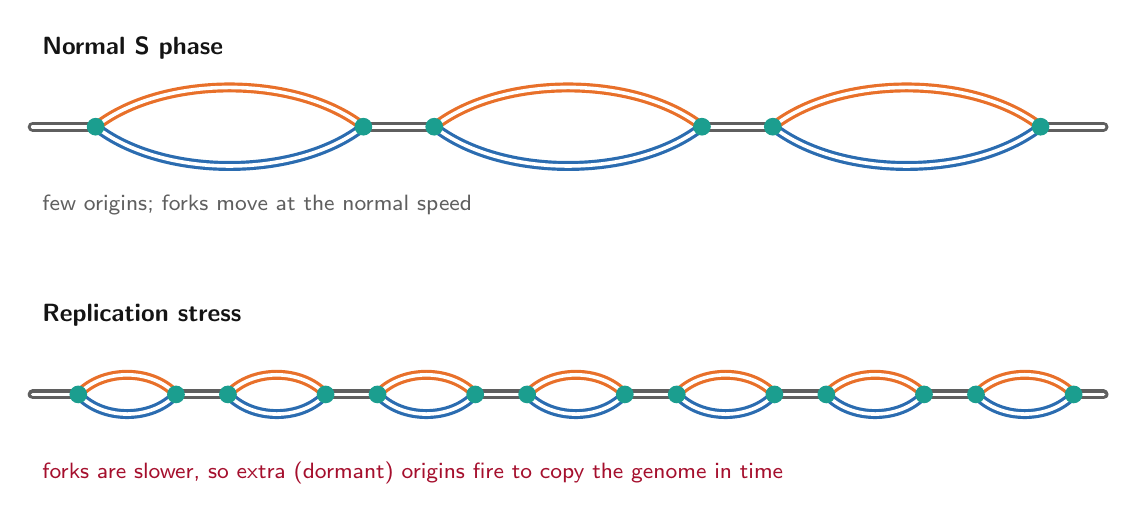
\begin{tikzpicture}[font=\sffamily\small,>=Stealth]
\node[ttl,anchor=west] at (-0.3,1.0) {Normal S phase};
\gseg{0}{-0.3}{0.5}\gseg{0}{3.9}{4.8}\gseg{0}{8.2}{9.1}\gseg{0}{12.5}{13.3}
\foreach \x in {2.2,6.5,10.8}{\eye{\x}{0}{1.7}{0.5}}
\node[lbl,anchor=west] at (-0.3,-1.0) {few origins; forks move at the normal speed};
\node[ttl,anchor=west] at (-0.3,-2.4) {Replication stress};
\gseg{-3.4}{-0.3}{0.28}\foreach \x in {0.9,2.8,4.7,6.6,8.5,10.4}{\gseg{-3.4}{\x+0.62}{\x+1.28}}\gseg{-3.4}{12.92}{13.3}
\foreach \x in {0.9,2.8,4.7,6.6,8.5,10.4,12.3}{\eye{\x}{-3.4}{0.62}{0.25}}
\node[lbl,anchor=west,red] at (-0.3,-4.4) {forks are slower, so extra (dormant) origins fire to copy the genome in time};
\end{tikzpicture}
\end{document}
